\documentclass{article}
\usepackage[utf8]{inputenc}
\usepackage[left=1cm,right=0.5cm,bottom=0.5cm,top=0.5cm]{geometry}
\usepackage{setspace}
\usepackage{graphicx}
\usepackage{amsmath}
\usepackage{enumitem}
\setstretch{0}
\setlist{nosep}

\begin{document}
\textbf{Resistors / current}
\begin{itemize}
    \item Series resistor | $R_{eq} = R_1 + R_2 + \dots + R_n$
    \item Parallel resistor | $\frac{1}{R_{eq}} = \frac{1}{R_1} + \frac{1}{R_2} + \dots \frac{1}{R_n}$
    \item Parallel resistors (2) | $R_{eq} = \frac{R_1R_2}{R_1 + R_2}$
    \item Voltage | $V = iR$
    \item Power | $p = vi = R^2i = \frac{v^2}{R}$
\end{itemize}
\textbf{Inductors / capacitors}
\begin{itemize}
    \item Cap current | $i = C \frac{dv}{dt}$ 
    \item Cap voltage | $v(t) = \frac{1}{C}\int_0^t i(t')dt'$
    \item Series cap | $\frac{1}{C_{eq}} = \frac{1}{C_1} + \frac{1}{C_2} + \dots \frac{1}{C_n}$
    \item Parallel cap | $C_{eq} = C_1 + C_2 + \dots + C_n$
    \item Cap time constant | $\tau = RC$
    \item Ind current | $i(t) = \frac{1}{L}\int_0^t v(t')dt'$
    \item Ind voltage | $v = L \frac{di}{dt}$
    \item Series ind | $L_{eq} = L_1 + L_2 + \dots + L_n$
    \item Parallel ind | $\frac{1}{L_{eq}} = \frac{1}{L_1} + \frac{1}{L_2} + \dots \frac{1}{L_n}$
    \item Ind time constant | $\tau = \frac{L}{R}$
\end{itemize}
\textbf{AC}
\begin{itemize}
    \item $Z_R = R$
    \item $Z_C = \frac{1}{C \omega j}$ | cap current leads voltage by $90^{\circ}$
    \item $Z_L = L \omega j$ | ind current lags voltage by $90^{\circ}$
    \item Capacitors are open circuit at DC, and voltage cannot change instantaneously.
    \item Inductors are short circuit at DC, and current cannot change instanteously.
    \item For "effectively charged to", calculate voltage and compare closest.
\end{itemize}
\textbf{Op-amps / diodes}
\begin{itemize}
    \item $v_o = A(v_p - v_n)$ | A is the gain (typically very large, unitless)
    \item $max(v_0) = |V_{cc}|$ | $V_{cc}$ is the power supply
    \item Diodes have bias: 
    \begin{itemize}
        \item If current is flowing forward, acts like a resistor. 
        \item If current is flowing backward, acts like an open circuit.
    \end{itemize}
    \item LEDs | diodes that emit light if voltage exceeds $V_{D,ON}$ or $V_F$. Also acts like a resistor.
    \item Negative feedback | allows linear range of op amps to be more usable (usually gain is too large)
\end{itemize}
\textbf{Ideal op-amps}
\begin{itemize}
    \item $i_p = i_n = 0$ | currents at negative / positive nodes are both 0.
    \item $v_p = v_n$ | both inputs are the same node.
    \item $A = R_i = \infty$ | gain and input op-amp resistance are infinite.
    \item $R_o = 0$ | output op-amp resistance is zero.
\end{itemize}
\textbf{MSP432}
\begin{itemize}
    \item Pins start from 0. Lowest bit is the 0th pin, highest bit is the 7th pin.
    \item \texttt{SEL0} and \texttt{SEL1} are mode select registers. Both 0 chooses GPIO for a certain pin.
    \item \texttt{DIR} sets the direction of the port's pins. 1 is out, 0 is in.
\end{itemize}
\textbf{SysTick Timer}
\begin{itemize}
    \item \texttt{LOAD} stores "max" value that timer is reset to.
    \item Timer counts down from \texttt{LOAD} to 0, then resets.
\end{itemize}
\textbf{TimerA}
\begin{itemize}
    \item Resolution = $T \cdot 2^{ID} \cdot (\texttt{TAIDEX} + 1)$
    \item Frequency = $\frac{f}{resolution}$
    \item \texttt{TA0CCR0} = max value for timer
\end{itemize}
\textbf{Pulse-width modulation}
\begin{itemize}
    \item $d = \frac{high}{period}$ | d = the duty cycle, period = \texttt{TA0CCR0}
\end{itemize}
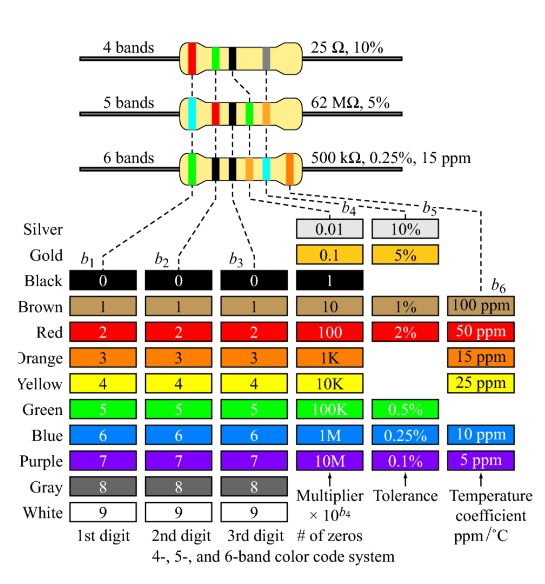
\includegraphics[width=10cm]{resistors.png}
\end{document}